%% BREAK LINES EVERY 80 CHARACTERS TO HELP GIT WITH MERGING
With the optimizations discussed in Section~\ref{ssec:precomputing}, 
pre-processing speeds increased dramatically from near-negligible time
to load the file to the times listed in Table~\ref{tab:precomputing}.
Note that there are only three entries per data set as pre-processing was 
done outside the |main()| function to save computation (\ie pre-processing
was done once for every 10 trials).
\begin{table}[h]
	\centering\small
	\def\arraystretch{1}
	\begin{tabular}{>{\bf}*4{c}} \hline 
		\textbf{Trial} & \textbf{Western Sahara} & \textbf{Uruguay} & \textbf{Canada} \\ \hline 
		1 & $112.342$ & $769.979$ & $31302.409$  \\
		2 & $110.887$ & $774.185$ & $30910.104$ \\
		3 & $110.485$ & $725.295$ & $30977.966$ \\ \hline 
	\end{tabular}
	\caption{Distance Pre-computation Times (ms)\label{tab:precomputing}}	
\end{table}
Execution of the GA was done with $5,000$ generations for each dataset 
with each generation taking approximately $400$, $1,200$, and $4,600$ 
milliseconds for Western Sahara, Uruguay, and Canada datasets, respectively.
For the smallest dataset, Western Sahara, $5,000$ proved to be a rather large 
number of iterations as the last generation with improved fitness hovers 
around $1,500$ (Table~\ref{tab:last-gen-tiny}). 
\begin{table}[H]
	\centering\small
	\tabcolsep=2pt
	\def\arraystretch{1}
	\begin{tabular}{*3{c}} \hline 
		\textbf{Trial} & \parbox{1.5cm}{\centering\bfseries Last\\Improve.} & \parbox{1.5cm}{\centering\bfseries Best\\Fitness} \\ \hline 
		1 & 1308 & 27620 \\
		2 & 4012 & 30664 \\
		3 & 2889 & 27768 \\
		4 & 3271 & 28513 \\
		5 & 4103 & 27768  \\
		6 & 3158 & 28202 \\
		7 & 1716 & 28202 \\
		8 & 1059 & 29154 \\
		9 & 1948 & 29098 \\
		10 & 2199 & 30048 \\
		11 & 4639 & 29177 \\
		12 & 1710 & 28039 \\
		13 & 839 & 27748 \\
		14 & 729 & 29686 \\
		15 & 597 & 29373 \\ \hline 
	\end{tabular}
	\begin{tabular}{*3{c}} \hline 
		\textbf{Trial} & \parbox{1.5cm}{\centering\bfseries Last\\Improve.} & \parbox{1.5cm}{\centering\bfseries Best\\Fitness} \\ \hline 
		16 & 1056 & 29337 \\
		17 &1407  & 27768 \\
		18 & 1686 & 28728 \\
		19 & 1078 & 28765 \\
		20 & 2371 & 28061 \\
		21 & 1534 & 28249 \\
		22 & 610 & 28735 \\
		23 & 4890 & 27620 \\
		24 & 2484 & 28249 \\
		25 & 803 & 29535 \\
		26 & 990 & 28231 \\
		27 & 1224 & 30709 \\
		28 & 810 & 30502 \\
		29 & 683 & 28222 \\
		30 & 4582 & 28755 \\ \hline 
	\end{tabular}
	\caption{Last Generation With Improvement (Western Sahara)\label{tab:last-gen-tiny}}
\end{table}
Consequently, Figure~\ref{fig:tiny-fitnesses} 
illustrates a plateau fairly early in the execution. This means that in 
some cases, similar results could be obtained much faster, with much
less computation. On the other hand, some trials have improvement 
as far as nearly $4,900$ generations into execution. Such trials sometimes
are the ones with the most optimal fitness (\eg trials $5$ and $23$
had improvement in generation $4,103$ and $4,890$, respectively 
and finished with best fitnesses of $27,768$ and $27,620$).
\begin{figure*}[h]
	\centering
	\fbox{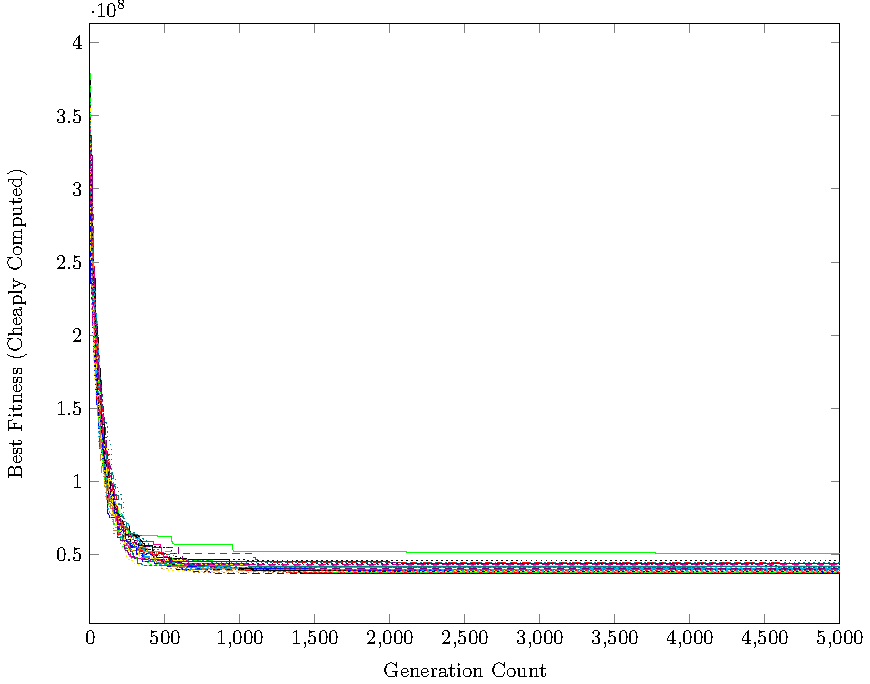
\includegraphics[width=0.65\linewidth]{include/graphs/fitness/tiny-fitnesses-lg}}
	\caption{Fitness Changes over $5,000$ Generations (Western Sahara)\label{fig:tiny-fitnesses}}
\end{figure*}
According to the University of Waterloo's Faculty of Mathematics, optimal fitness for this tour is $27,603$ \cite{sahara}. Therefore, several of the trials logged in Table~\ref{fig:tiny-fitnesses} show the algorithm's effectiveness in reaching near-optimal solutions. Given time to run more generations, optimal solutions should be achieved.

Uruguay, on the other hand, did not plateau in the same way that 
Western Sahara did (Figure~\ref{fig:med-fitnesses}).
\begin{table}[H]
	\centering\small
	\tabcolsep=2pt
	\def\arraystretch{1}
	\begin{tabular}{*3{c}} \hline 
		\textbf{Trial} & \parbox{1.5cm}{\centering\bfseries Last\\Improve.} & \parbox{1.5cm}{\centering\bfseries Best\\Fitness} \\ \hline 
		1 & 4995 & 682092 \\
		2 & 4987 & 686624 \\
		3 & 4991 & 675225 \\
		4 & 4993 & 675225 \\
		5 & 4974 & 685579  \\
		6 & 4990 & 673494 \\
		7 & 4996 & 689418 \\
		8 & 4996 & 678421 \\
		9 & 4995 & 659951 \\
		10 & 4999 & 687908 \\
		11 & 4987 & 680266 \\
		12 & 4988 & 699569 \\
		13 & 4998 & 702853 \\
		14 & 4993 & 696526 \\
		15 & 4995 & 701105 \\ \hline 
	\end{tabular}
	\begin{tabular}{*3{c}} \hline 
		\textbf{Trial} & \parbox{1.5cm}{\centering\bfseries Last\\Improve.} & \parbox{1.5cm}{\centering\bfseries Best\\Fitness} \\ \hline
		16 & 4993 & 687626 \\
		17 &4996  & 683809 \\
		18 & 4989 & 691854 \\
		19 & 4995 & 705421 \\
		20 & 4995 & 672055 \\
		21 & 4996 & 686104 \\
		22 & 4967 & 685925 \\
		23 & 4990 & 674031 \\
		24 & 4981 & 687605 \\
		25 & 4999 & 707432 \\
		26 & 4991 & 681644 \\
		27 & 4995 & 671644 \\
		28 & 4987 & 702787 \\
		29 & 4993 & 690934 \\
		30 & 4999 & 694009 \\ \hline 
	\end{tabular}
	\caption{Last Generation With Improvement (Uruguay)\label{tab:last-gen-med}}
\end{table}
\begin{figure*}[h]
	\centering
	\fbox{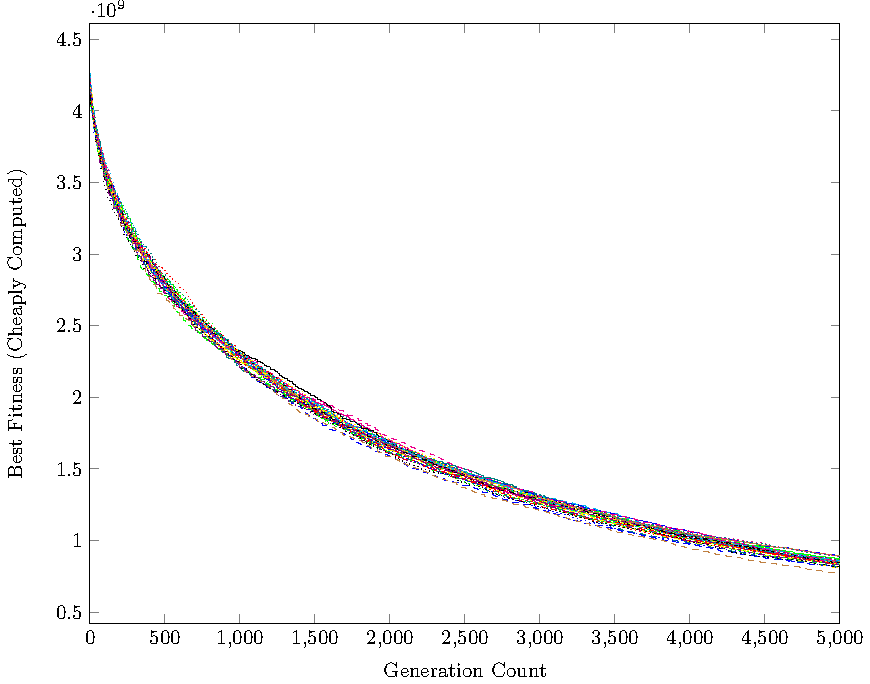
\includegraphics[width=0.65\linewidth]{include/graphs/fitness/med-fitnesses-lg}}
	\caption{Fitness Changes over $5,000$ Generations (Uruguay)\label{fig:med-fitnesses}}
\end{figure*}
This can be seen both by the way that Figure~\ref{fig:med-fitnesses}
maintains a relatively steep slope all the way to the last generation, 
as well as the high frequency of improvements above $4,980$ generations in
Table~\ref{tab:last-gen-med}.
Consequently, the algorithm, given more time to compute more generations,
should yield similar results as were demonstrated for Western Sahara.

Execution for the Canada dataset ran successfully for a number of trials,
however, due to the technique of running ten trials of the algorithm per execution,
technical errors mid-way through execution spoiled the data for all trials. 